\chapter{Rotational Motion and Frictional Losses}

Date: 29/11/2020

\section{Aim}

The aim of this experiment is to understand energy losses due to frictional. We will study the relationship between frictional losses in 
a pulley and mass of the object.
    
%An aim is a short description of what you are about to do in the experiment. It usually answers the questions like, 
%\begin{enumerate}
 %   \item What are you plan on doing?
 %  \item How are you doing it?
  %  \item Why are you doing it?
%\end{enumerate}


\section{Background Theory}

%This section is meant to explain the theoretical background of the experiment whose report you are writing. Theoretical background does not mean historical background. Be precise to, ONLY include scientific background.

Consider the provided circular disks (rigid bodies) to be made up of small infinitesimal particles of masses $m_1,m_2,m_3, \cdots,m_n$. Their placement may be defined with the position vectors $\vec{r_1},\vec{r_2},\cdots.\vec{r_n}$ and when rotating, their instantaneous velocities may be defined as
$\vec{v_1},\vec{v_2},\vec{v_3} ,\cdot,\vec{v_n}$.
The angular momentum of a particle given is by
\begin{equation}
    \label{eq1}
    \vec{J_i} = m \vec{v_i} \times \vec{r_i}
\end{equation}
For a particle rotating with angular velocity 
$ \omega$ about z axis, we can say that
\begin{equation}
    \label{eq2}
    v_i = r_i \omega_i
\end{equation}
We can then combine \ref{eq1} and \ref{eq2} to obtain the following equation
\begin{equation}
    \vec{J_i} = m\vec{r_i}\vec{\omega_i}
\end{equation}
Then the total angular momentum of the disk is simply the sum of the angular momentum of the individual particles making the disk.
\begin{equation}
    \vec{J} = \sum_i^n  m\vec{r_i}^2\vec{\omega_i}
\end{equation}
The quantity $\sum_i^n  m\vec{r_i}^2$ is known as moment of Inertia I. In this form , the angular momentum of the disc becomes
\begin{equation}
    J_z = \omega I
\end{equation}
We can write I in the similar form as transalational moment,
\begin{equation}
    I = \frac{1}{2} M R^2
\end{equation}
Rotational Kinetic energy is defined as 
\begin{equation}
    K = \frac{1}{2} I \omega ^2
\end{equation}
Moment of inertia of a particular body is defined with respect to a particular rotation axis and is different for a body when it is rotating about x, y or z axes.







\section{Description of Setup}
\newpage
\begin{figure}[h!]
   \centering
    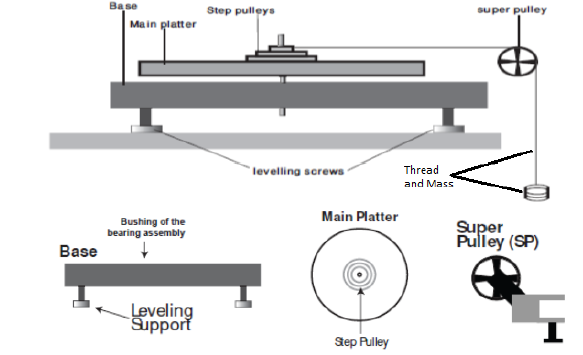
\includegraphics[width=\textwidth]{figures/Apparatus11.png}
    \caption{Apparatus and the arrangement of the experimental setup.}
    \label{fig:yx}
\end{figure}
Here the base is used to hold the platters and pulleys, main platter is the object which is performing the Rotational motion, camera and metre are used in conjunction to measure the height of the hanging mass, step pulley is used to adjust the torque , super pulley is used to provide a smooth transition from Translation to Rotational Motion and the Thread ans Mass are used to execute Translation Motion and rotate the main platter.

%Sketch and explain the experimental setup. The explanation should try to cover these pointers: 
%\begin{enumerate}
%   \item What is the purpose of individual items in the setup?
%   \item If any equipment is taking measurements, what is it reading and how is it being read?
%\end{enumerate}

%Be precise to, ONLY include scientific description.

\section{Method / Procedure}

%Highlight the following aspects of the experiment conducted 
%\begin{enumerate}
%   \item What method did you use to perform the experiment?
%   \item What adjustments were made, if any? 
%   \item What data was collected?
%    \item How was it collected?
%    \item Were any calibrations made and what were they?
%\end{enumerate}

%Be precise to, ONLY include scientific background.

In the given experimental setup, the thread is wrapped about the spindle as the wheel is spun. This lifts the mass tied to the other end of the thread by some distance, thereby storing potential energy in it. The disk is released, and the mass is let to oscillate for about five cycles, recording the height of the mass as a function of time.The same experiment using is for three other masses four masses. Then a graph of potential energy vs time is plotted in MATLAB for each particular value of Mass.

\section{Data}
The type B uncertainty in the height h is $0.001m$, in the time t is $0.003s$ and in the mass is $0.00003kg$.

\begin{center}
\begin{tabular}{|l|l|l|l|l|l|}
\hline
\multicolumn{6}{|c|}{\textbf{Mass (grams) = 23.3}} \\ \hline
\textbf{s.No} & \textbf{Time (s)} & \textbf{Max\_h (cm)} & \textbf{Min\_h (cm)} & \textbf{Diff\_h (cm)} & \textbf{P.E(J)} \\ \hline
0   & 0       & 68     & 12   & 56    & 0.1280009  \\ \hline
1   & 17.37   & 60     & 12   & 48    & 0.109715   \\ \hline
2   & 33.41   & 52     & 12   & 40    & 0.0914292  \\ \hline
3   & 48.09   & 45.5   & 12   & 33.5  & 0.076572   \\ \hline
4   & 62.37   & 40     & 12   & 28    & 0.0640004  \\ \hline
5   & 73.81   & 35.5   & 12   & 23.5  & 0.0537147  \\ \hline
\end{tabular}
\end{center}
\begin{center}
\begin{tabular}{|l|l|l|l|l|l|}
\hline
\multicolumn{6}{|c|}{\textbf{Mass (grams) = 43.0}} \\ \hline
\textbf{s.No} & \textbf{Time (s)} & \textbf{Max\_h (cm)} & \textbf{Min\_h (cm)} & \textbf{Diff\_h (cm)} & \textbf{P.E(J)} \\ \hline
0   & 0       & 68     & 12   & 56     & 0.236225  \\ \hline
1   & 12.21   & 62.5   & 12   & 50.5   & 0.219352  \\ \hline
2   & 24.12   & 56.5   & 12   & 44.5   & 0.202478  \\ \hline
3   & 35.71   & 51.5   & 12   & 39.5   & 0.183496  \\ \hline
4   & 46.89   & 46.5   & 12   & 34.5   & 0.166623  \\ \hline
5   & 57.16   & 43     & 12   & 31     & 0.153968  \\ \hline
\end{tabular}
\end{center}
\begin{center}
\begin{tabular}{|l|l|l|l|l|l|}
\hline
\multicolumn{6}{|c|}{\textbf{Mass (grams) = 62.6}} \\ \hline
\textbf{s.No} & \textbf{Time (s)} & \textbf{Max\_h (cm)} & \textbf{Min\_h (cm)} & \textbf{Diff\_h (cm)} & \textbf{P.E(J)} \\ \hline
0   & 0       & 68     & 12   & 56    & 0.3438994  \\ \hline
1   & 10.02   & 63.5   & 12   & 51.5  & 0.3162646  \\ \hline
2   & 20.27   & 58.5   & 12   & 46.5  & 0.2855593  \\ \hline
3   & 30.31   & 54     & 12   & 42    & 0.2579245  \\ \hline
4   & 39.43   & 50     & 12   & 38    & 0.2333603  \\ \hline
5   & 48.86   & 46.5   & 12   & 34.5  & 0.2118666  \\ \hline
\end{tabular}
\end{center}

\begin{center}
\begin{tabular}{|l|l|l|l|l|l|}
\hline
\multicolumn{6}{|c|}{\textbf{Mass (grams) = 82.2}} \\ \hline
\textbf{s.No} & \textbf{Time (s)} & \textbf{Max\_h (cm)} & \textbf{Min\_h (cm)} & \textbf{Diff\_h (cm)} & \textbf{P.E(J)} \\ \hline
0   & 0       & 68     & 12   & 56     & 0.451574  \\ \hline
1   & 9.2     & 64     & 12   & 52     & 0.419319  \\ \hline
2   & 18.45   & 60     & 12   & 48     & 0.387063  \\ \hline
3   & 27.09   & 55.5   & 12   & 43.5   & 0.350776  \\ \hline
4   & 35.54   & 51.5   & 12   & 39.5   & 0.318521  \\ \hline
5   & 43.62   & 48.5   & 12   & 36.5   & 0.294329  \\ \hline
\end{tabular}
\end{center}
%In this section, describe what data was recorded during the experiment. Mention which quantities are being measured, which quantity is independent, which is dependent and which are constants. Make this difference very explicit. Make sure to quantify and state the uncertainties in the recorded data. Be precise and primarily include numerical data.

\section{Data Analysis}

%In this section, mention the calculations you perform, uncertainties transferred, and statistical analysis (residuals, errors, uncertainties in parameters fit etc.). Be precise and primarily include numerical data.
Values obtained by curve Fitting of Potential Energy vs Time using the equation $ a \times e^{bt}$ are summarised in the following table.
\begin{center}
\begin{tabular}{|l|l|l|l|}
\hline
\multicolumn{4}{|c|}{Curve   Fitting Results} \\ \hline
s.No   & Mass(gram)   & a        & b (Frictional Loss Coefficient  )       \\ \hline
1      & 23.3         & 0.1305   & -0.01131   \\ \hline
2      & 43           & 0.2389   & -0.01034   \\ \hline
3      & 62.6         & 0.3467   & -0.00992   \\ \hline
4      & 82           & 0.4645   & -0.00986   \\ \hline
\end{tabular}
\end{center}

\begin{figure}[h!]
   \centering
    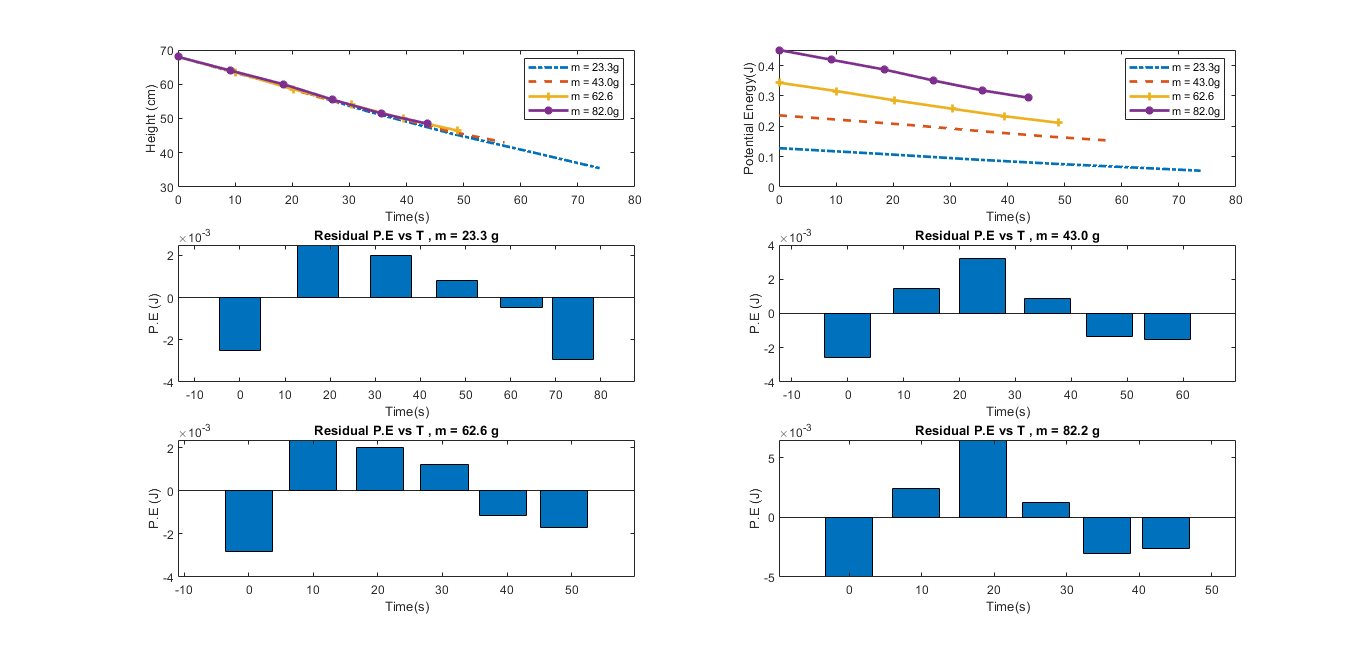
\includegraphics[width=1\textwidth]{figures/AllPlots.png}
    \caption{Graph of Height, Potential Energy vs Time and Residual Plots}
    \label{fig:yx}
\end{figure}



\newpage
\begin{figure}[h!]
   \centering
    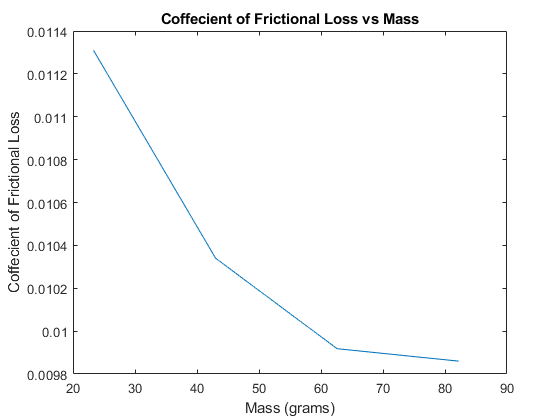
\includegraphics[width=\textwidth]{figures/frictional.png}
    \caption{Graph of coefficient of Frictional Loss vs Mass}
    \label{fig:yx}
\end{figure}

\section{Discussion \& Conclusion}

%Summarize and discuss the experimental results, what do the results say about your hypothesis, if such a hypothesis was made for the experiment. Mention the uncertainty in the calculated quantity Be precise and only include scientific discussion.

The fit plot of Potential Energy vs Time is decreasing exponentially which is what we expected . Due to energy loss to friction, the maximum height decreased in each cycle and this turn meant that the potential energy decreased and we observed this in the plot. The graph of coefficient of frictional loss  vs mass has an increasing trend which means that more larger the mass , greater the energy loss. Sinusoidal pattern in the residual indicates the presence of random error. One way to improve these errors is to take more readings which can be done by taking more values of masses and recording maximum height for more cycles. 


\section{MATLAB Script}
\lstinputlisting{matlabCodes/Experiment11.m}



